\chapter{Тестирование и апробация пакета} \label{ch4}

% не рекомендуется использовать отдельную section <<введение>> после лета 2020 года
%\section{Введение} \label{ch4:intro}

Хорошим стилем является наличие введения к главе. Во введении может быть описана цель написания главы, а также приведена краткая структура главы. 
	
\section{Проверка установки пакета} \label{ch4:sec}

В первую очередь была написана инструкция по установке и удалению, и помещена к инсталлеру. После чего был протестирован скрипт создания пакета и его удаления. Замеченные недостатки устранялись, на данном этапе была поправлена последовательность создания и удаления объектов. Была проверена установка значений параметров по умолчанию, в ходе тестирования были модифицированы некоторые значения параметров, для максимального быстродействия. 

\section{Проверка работы пакета} \label{ch4:sec2}

Для тестирования пакета был написан скрипт, содержащий тестовые случаи, который был добавлен к скрипту установщику. Была проверена работа всех, объявленных в спецификации пакета, процедур и функций в различных ситуациях и с разными настройками пакета. Рассматривались как положительные случаи, так и отрицательные ситуации (некорректные данные, отсутствующие данные). Часть тестов была автоматизирована, часть оставлена для ручной проверки. Автоматические тесты выполняют несколько ситуаций и сравнивают результат с эталоном, после чего выводят на экран результат проверки. 

На рисунке \firef{fig:c4_auto_test} представлена часть кода автоматических тестов. 

\begin{figure}[ht!] 
	\center
	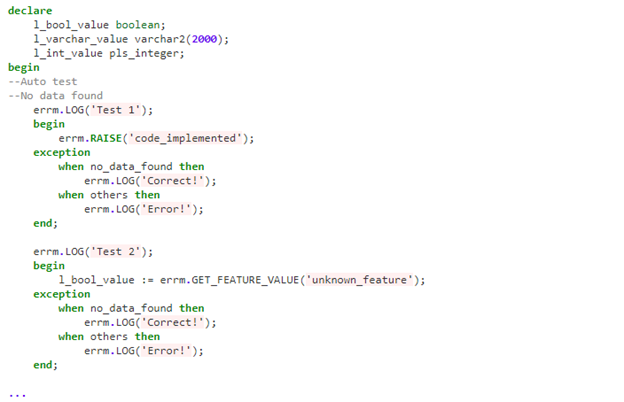
\includegraphics [scale=1] {my_folder/img/c4_auto_test.png}
	\caption{Пример кода автоматических тестов} 
	\label{fig:c4_auto_test}  
\end{figure}
\FloatBarrier

Первый тест проверяет вызов несуществующий ошибки по ее имени. Второй, пытается получить значение опции, по имени, которое не содержится в таблице ERRM\$FEATURE\_FLAGS. 

Остальные автоматические тесты проверяют следующие ситуации.

Тест 3 устанавливает значение несуществующей опции.

Тест 4 устанавливает значение параметра, которого не существует.

Тест 5 пытается получить значение отсутствующего параметра.

В тесте 6 проверяется ситуация получения кода ошибки, которая не определена.

Вызов ошибки с несуществующим кодом проводится в тесте 7.

Тест 8 повторяет 7 тест, но запрещает логирование.

Тест 9 вызывает ошибку по имени, которой не существует.

Тест 10 делает тоже самое, но без логирования.

Тесты 11 и 12 проверяют методы SRAISE с кодом и именем не существующих ошибок, соответственно. 
Каждый тест обернут в блок begin\/end с обработчиком ошибки, если возникла правильная ошибка, тест возвращает корректный результат, если возникла другая ошибка, тест сообщает о неудаче. 

9 ручных тестов предназначены для проверки корректности работы основных методов, а также некоторых параметров и опций пакета.

\begin{figure}[ht!] 
	\center
	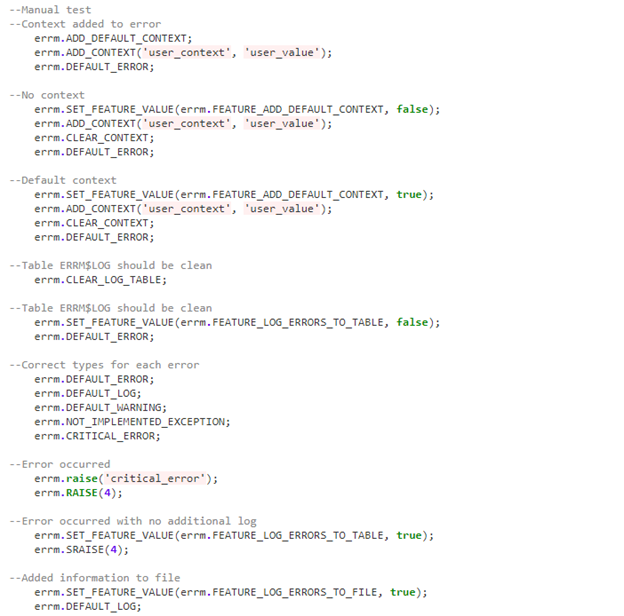
\includegraphics [scale=1] {my_folder/img/c4_manual_test.png}
	\caption{Код для ручного тестирования пакета} 
	\label{fig:c4_manual_test}  
\end{figure}
\FloatBarrier

На рисунке \firef{fig:c4_manual_test} представлены ручные тесты. Каждый случай содержит комментарий с описанием ожидаемого результата.

Первая ситуация проверяет добавление контекста к ошибке.
 
Второй тест проверяет возможность очистки контекста. 

Третий тест демонстрирует как должна работать очистка контекста, в ситуации с автоматическим добавлением стандартного контекста. 

Четвертый тест проверяет корректность очистки таблицы логирования.

Тест под номер пять проверяет флаг для отключения логирования в таблицу. 

Тест 6 состоит из вызова нескольких предопределенных ошибок, здесь проверяется корректность типов ошибок, и в целом работа всей системы.

Тест 7 проверяет вызов ошибки по имени и коду.

Тест 8 проверяет корректность работы методов «тихого» вызова исключения. 

Тест 9 проверяет запись в файл логирования. 

Помимо этого, была проверена запись логов в файл, корректность отработки внутренних (скрытых от пользователя в теле пакета) методов, были проверены ситуации добавления значений в контекст с одинаковым ключом, множественное добавление базового контекста и некоторые другие случаи.

Все найденные в ходе тестирования ошибки и недочеты исправлялись. 

Не удалось настроить работу почтового сервиса на виртуальной машине, поэтому тестирование отправки Email сообщение провалилось. Данная опция была отключена по умолчанию. 

\section{Улучшение кода} \label{ch4:sec3}

Во время проверки составлялся список субъективных ощущений от работы с пакетом, после чего данный список был проанализирован, неудобства в работе с пакетом скорректированы. 

Был проведен рефакторинг с целью улучшения работы пакета. В ходе него были удалены неиспользуемые переменные и методы, были устранены некоторые узкие места, были пересмотрены используемые типы данных, и сигнатуры некоторых методов.

После рефакторинга было проведено дополнительно полное тестирование пакета, с целью выявление регресса. Найденные проблемы были устранены. 


\section{Сравнение полученных результатов} \label{ch4:sec4}

На рисунке \firef{fig:c4_examples} представлены три примера кода, работающего с исключительными ситуациями. 

\begin{figure}[ht!] 
	\center
	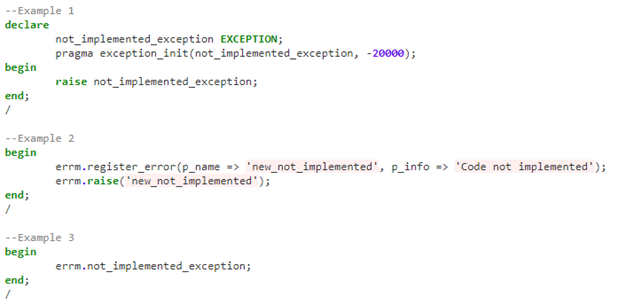
\includegraphics [scale=1] {my_folder/img/c4_examples.png}
	\caption{Примеры использования пакета} 
	\label{fig:c4_examples}  
\end{figure}
\FloatBarrier

Пример 1 использует стандартные средства для вызова исключения. Пример 2 объявляет новое исключение при помощи пакета, а затем вызывает его. Пример 3 вызывает существующее исключение. 

Второй код больше приближен к первому примеру, так как создается новое исключение, и выигрыш в объеме кода является не таким значимым, первый случай содержит 150 символов, в то время как во второй ситуации только 136, но второй пример имеет значительный выигрыш в других показателях. 

Результаты выполнения первого примера показаны на рисунке \firef{fig:c4_1_example_res}:

\begin{figure}[ht!] 
	\center
	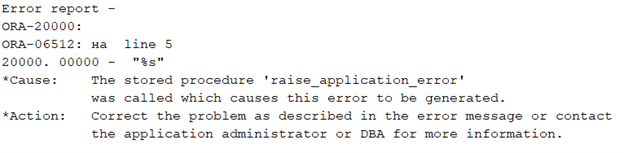
\includegraphics [scale=1] {my_folder/img/c4_1_example_res.png}
	\caption{Результаты выполнения первого примера} 
	\label{fig:c4_1_example_res}  
\end{figure}
\FloatBarrier

На рисунке \firef{fig:c4_2_example_res} представлены результаты выполнения второго кода:

\begin{figure}[ht!] 
	\center
	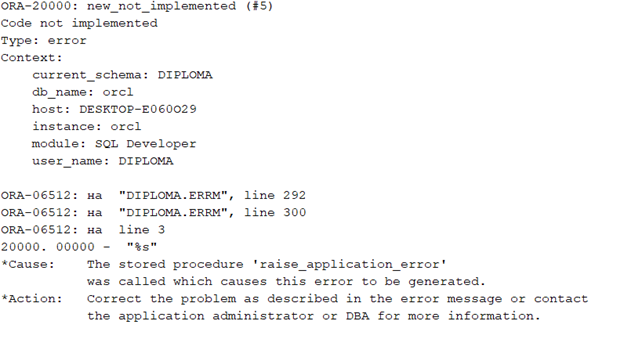
\includegraphics [scale=1] {my_folder/img/c4_2_example_res.png}
	\caption{Результаты выполнения второго примера} 
	\label{fig:c4_2_example_res}  
\end{figure}
\FloatBarrier

В первом случае мы не получили никакой информации об ошибке, сообщение пустое, почему возникло исключение в коде не понятно. В то время второй код, содержит описание об возникшей ошибке (которая только что создана), а также дополнительную мета информацию, помимо этого сообщение об ошибке будет занесено в таблицу логирования, и в файл логов. Созданная ошибка сразу будет видна другим исполняемым блокам, в то же время информация об ошибке в первом примере доступна только самому анонимному блоку и его вложенным блокам. 

Созданную ошибку можно заново использовать без дополнительного кода. Нет необходимости следить за кодами ошибок. Информацию обо всех существующих ошибках можно легко узнать из одной таблицы ERRM\$ERRORS. 

Пример под номером три, показывает работу пакета в более реальной ситуации, обычно мы хотим использовать уже известную исключительную ситуацию, для часто используемых ошибок, достаточно вызвать единственный метод без параметров. При этом мы получим результат подобный примеру 2, и соответственно все его преимущества. Третий пример состоит всего из 44 символов, следовательно мы потратим меньше времени на написание кода, а важнее то, что нам не потребуется выполнять дополнительные действия для простых ситуаций. 

Следующий пример, представленный на рисунке \firef{fig:c4_add_context_example}, демонстрирует использование контекста для сохранения значений параметров.

\begin{figure}[ht!] 
	\center
	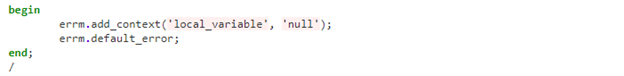
\includegraphics [scale=1] {my_folder/img/c4_add_context_example.png}
	\caption{Пример добавления контекста} 
	\label{fig:c4_add_context_example}  
\end{figure}
\FloatBarrier

В результате выполнения этого скрипта, в сообщение об ошибке (а также во всех местах куда логируется информация, согласно настройкам) будет содержаться указанная нами информация, что в перспективе облегчит отладку, и исправление ошибки. 

Указанные выше примеры, а также некоторые дополнительные, были объединены в один скрипт, который будет распространяться вместе с пакетом для демонстрации различных возможностей приложения.



\section{Выводы} \label{ch4:conclusion}

В данной главе было проведено тестирование кода, а также его улучшение и настройка. Были приведены примеры работы с пакетом, а также сравнение разработанного пакета в работе со стандартным способом. 
